\section{Position Calculations}\label{sec:position-calculations}
In order to develop a game where a user moves to control the game, it is necessary to register these movements and calculate a position. 
Calculating positions can be done by analysing the data given from the accelerometer in the phone.
The output of the accelerometer is the accelerations of the three axis' of the accelerometer.
\figref{figure:acceleration-chart} and \figref{figure:velocity-chart} shows two graphs with each graph showing three steps.
\figref{figure:acceleration-chart} is the acceleration along the y-axis of the phone. 
\figref{figure:velocity-chart} is the velocity along the y-axis of the phone.
The velocity is calculated by taking the integral of the acceleration, the formula is as follows:
\begin{equation*}
v(T) = \int_0^T \! a(t) \, \mathrm{d}t
\end{equation*} 
where, $v(T)$ is the velocity at time $T$, and $a(t)$ is the acceleration at time $t$.

A graph with accelerations and a graph with the corresponding velocities can be seen in \figref{figure:acceleration-chart} and \figref{figure:velocity-chart}, respectively.

\begin{figure}[H]
	\centering	
	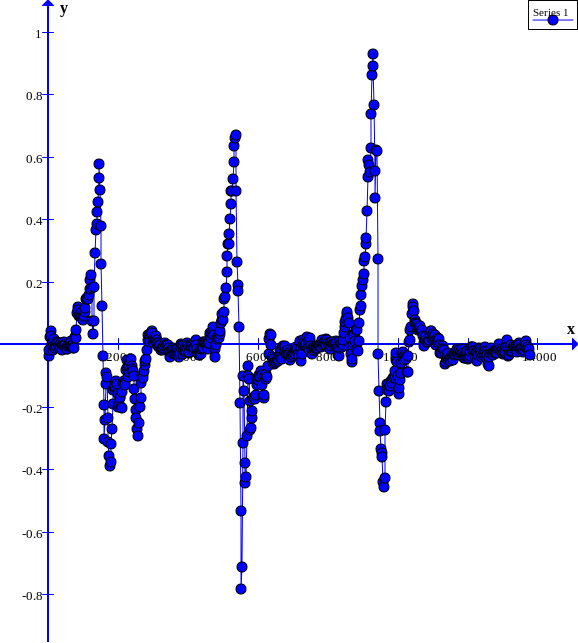
\includegraphics[scale=0.4, trim=0cm 2cm 0cm 2cm]{media/gnuplot/acceleration.pdf}
	\caption{Acceleration readings over three steps.}
	\label{figure:acceleration-chart}
\end{figure}

\begin{figure}[H]
	\centering	
	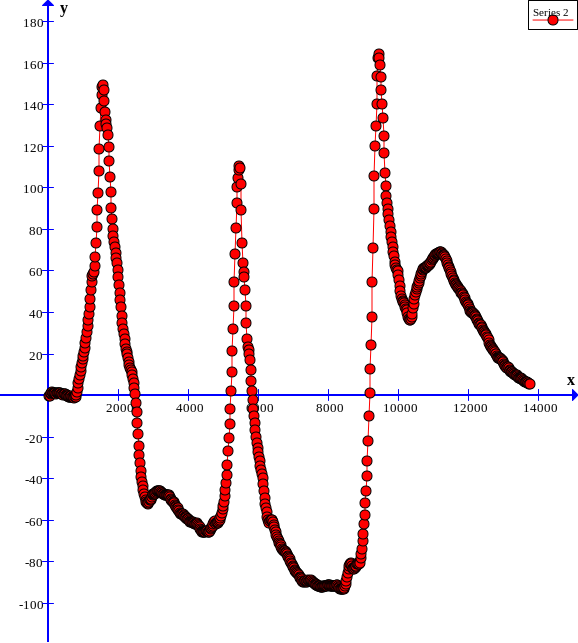
\includegraphics[scale=0.4, trim=0cm 2cm 0cm 2cm]{media/gnuplot/velocity.pdf}
	\caption{Velocity calculations over three steps.}
	\label{figure:velocity-chart}
\end{figure}

The velocity graph is smoother than the acceleration graph because each point on the velocity graph is a summation of the area of the acceleration graph.

To determine the position, the area under the velocity graph is calculated by taking the integral of the velocity over time, as seen in the following equation:

\begin{equation}\label{eq:integral-velocity}
     s(T) = \int_0^T v(t)\mathrm{d}t 
\end{equation}
where, $s(T)$ is the distance at time $T$, and $v(t)$ is the velocity at time $t$. 

The value can be used in conjunction with the previous position to calculate an approximation of the new position.
The actual values can be observed by video footages of people sidestepping with the phone.
As seen in the graphs, noise exists and should be corrected by use of filters.